\documentclass{article}[12pt]
\usepackage{graphicx}
\usepackage{tabularx}
\usepackage{natbib}

\usepackage{array}
\usepackage{amsmath}
%\usepackage[backend=bibtex]{biblatex}
\bibliographystyle{..//refs/styles/ecoletters.bst}
\setkeys{Gin}{width=0.8\textwidth}
%\setlength{\captionmargin}{30pt}
\setlength{\abovecaptionskip}{10pt}
\setlength{\belowcaptionskip}{10pt}
 \topmargin -1.5cm 
 \oddsidemargin -0.04cm 
 \evensidemargin -0.04cm 
 \textwidth 16.59cm
 \textheight 21.94cm 
 \parskip 7.2pt 
\renewcommand{\baselinestretch}{2}
\AtBeginEnvironment{thebibliography}{\linespread{1}\selectfont}
\parindent 0pt
\usepackage{lineno}
\linenumbers % for dissertation

%\usepackage{xr-hyper}
%\usepackage{hyperref}


\title{Phenological differences among species explain why early leafout extends the calendar but not thermal growing season}
%dl2024Sept20: I like the idea here, but struggle with the wording---"extends the calendar"--- it might be confusing to a reader unfamiliar with the concept

\author{D.M. Buonaiuto $^{1,2,3}$, C.J. Chamberlain $^{2,3,4}$,
Deirdre Loughnan$^{5}$, E.M. Wolkovich$^{2,3,5}$}

\usepackage{Sweave}
\begin{document}
\Sconcordance{concordance:phen_framing.tex:phen_framing.Rnw:1 35 1 1 0 18 1 1 112 181 %
1}



\maketitle

\noindent \emph{Author affiliations:}\\
\noindent $^1$Department of Plant Science and Landscape Architecture, University of Maryland, College Park, Maryland, USA. ORCID: 0000-0003-4022-2591\\
\noindent $^2$Arnold Arboretum of Harvard University, Boston, Massachusetts, USA.\\
$^3$Department of Organismic and Evolutionary Biology, Harvard University, Cambridge, Massachusetts, USA \\
$^4$The Nature Conservancy, Cat should add, USA \\
$^5$Forest \& Conservation Sciences, Faculty of Forestry, University of British Columbia, Vancouver, British Columbia, Canada\\
$^a$Corresponding author: 301.405.1061; dbuona@umd.edu\\


%\setlength{\parskip}{0.5pt} % 1ex plus 0.5ex minus 0.2ex}
\setlength{\parindent}{0pt}

%cjc2024Sept25: I think Lizzie and Deirdre already hit the highlights for the Intro for now. I agree that there are paragraphs that need to be moved to the Results and Discussion (anything that includes the figures). I also think you need to set up the experiment a bit better in why it's so cool. A little more development on the latitudinal gradient would be good, even if the results aren't exciting, it'd be great to set up our initial hypothesis more. And maybe get into trees vs shrubs and interannual variation. This was a massive endeavor, I want the reader to be excited about it. 



\section{Abstract}
% emwJuly22: I can make more edits to abstract when we have a journal in mind and thus a length
The extension of the growing season in the spring in temperate regions is one the most prominent biological indicators of climate change. Most models of carbon storage assume that earlier seasons will result in longer seasons and thereby enhance forest carbon storage, however current findings have challenged this assumption.

A recent hypothesis that has gained support in the literature is that plants dynamically adjust the end of their growing season based on their carbon-sink capacity, such that longer seasons do not increase total productivity. If this is the case, variation in the calendar growing season (number of days) should be independent of variation in the thermal growing season (i.e., the period of favorable meteorological conditions for plant growth), which should remain relatively stable across years. % emwJuly22: I really like this but we need to mirror the language below for the readers. Right now a reader cannot follow how the 'unexpected trade-off' relates to this. We probably need to move and change the language below of 'This relationship may explain some of the contrasting results of how climate change affects growing season length and productivity.' 
We tested this prediction using rarely available plant-scale phenological measurements from a three year common garden experiment. The garden included 18 woody species, native to the Eastern United States from four populations of origin. 

We found an unexpected trade-off between early calendar growing seasons and thermal growing seasons in which delayed leafout in calendar time resulted in a longer thermal growing season---a relationship that was strongest in early-leafing species. At the community level, earlier leafout was correlated with earlier budset, resulting in a relatively stable calendar growing period over the three years. 
% emwJuly22: If we keep the below sentence we need to spell it out more easily for readers. 
Earlier leafout may have little advantage to the thermal growing season because early lower temperature are less favorable for photosynthesis, and the correlation between leafout and budset suggest early individuals will miss out on later-season conditions more favorable for photosynthesis. This relationship may explain some of the contrasting results of how climate change affects growing season length and productivity. This study shows linking phenological growing seasons to carbon storage requires integrating existing ecosystem measures with phenological variation at multiple scales, and that progress will require more efforts to understand and model species-level shifts in phenology.

\section{Introduction}
%cjcJan6 - Added tweaks to the first line but I don't know a lot of great info for the other sentences here
Terrestrial forests currently sequester 20\% of greenhouse gas emissions annually  \citep{shanley2024, roe2021}, providing a significant mitigation pathway for climate change. In mid and high latitudes, net carbon uptake is primarily determined by the length of the growing season \citep{White1999}. Most models of carbon storage assume that earlier spring leafout with climate change will drive longer seasons and increased carbon storage, in part offsetting future warming \citep{Churkina2005,White1999,Keenan2014}. Current findings, however, have called this major assumption into question. Recent research has suggested that plants adjust their end of season timing dynamically such that longer seasons do not increase total productivity, but the mechanism---and prevalence---of this effect is unclear \citep{Zani2020,Norby2021,Zohner2023}.

%emwNov4 -- I would love to get Cat's help on citations in this paragraph (and throughout). I have offered some, but her ideas would be better.
Some of this uncertainty may stem from the fact that there are multiple ways to measure the growing season \citep{Korner2023}. The most common is calendar time (i.e., the number of days between the start and end of the growing season). Observations have found that calendar growing seasons have lengthened with climate change \citep{Menzel1999,Liu2010}, but other studies have found that earlier leafout is often correlated with earlier end-of-season events \citep{Zani2020,Liu2016,Keenan2015}. % emwJuly22: The contrast in the sentence above needs a smidge of work -- you contrast 'observations' versus 'other studies' so it needs to either be 'some studies ... other studies' (or 'earlier studies... recent studies') or (better) contrast methods (ground observations vs satellites and experiments, or such ... actually, if possible, this would place to refer to scale issues). 

The thermal growing season---defined here as the period of favorable meteorological conditions for plant growth \citep{Korner2023}---offers an alternative to the calendar growing season. It is also widely used, most commonly in the metric of growing degree days, a temperature derived measure of time that accumulates when temperatures are above a certain minimal threshold \citep{CHUINE2000337,Moore:2014wl,YANG199561}. Because plant photosynthetic rates increase with temperature \citep{Farquhar:1980vm} the thermal growing season is mechanistically related to primary productivity, and thus may be a better proxy than calendar time for relating growing season length to carbon gain. Importantly, depending on the temperature over the course of a growing season, years with substantially different calendar growing seasons can have very similar thermal growing seasons, or \emph{vice versa}.

Recent work has suggested early, increased productivity in the calendar growing season drives early senescence \citep{Zani2020}, and proposed that plants adjust mid-season based on a combination of growing season temperature and daylength \citep{Zohner2023}, thus maintaining a consistent thermal growing season. Such studies, however, are based generally on large-scale satellite measurements and small-scale single species `pot' experiments, and contrast with findings from long-term large-scale $CO_2$ enrichment studies \citep{norby2021comment}.

% emwJuly22: This paragraph has a lot of good stuff in it but needs some flow. The first sentence is good, but then you jump to satellites, when instead you should set up spatial scale issues here (or can you hint at it above at all? I pointed out one spot or just the previous sentence with 'pot' effects should do it if you make th connection better for the reader)
These contrasting results suggest fundamental gaps in our understanding of how early-season events, and the thermal conditions of the vegetative period, shape end-of-season events. While results from satellite-derived metrics of phenology (e.g., using NDVI) show a correlation between the start and end of the season, the signature that is measured for `end of season' is not clearly tied to a plant-scale event. Yet any connections would likely start at the individual plant level, where we rarely, if ever, have good measures of start and end of season events together. Further, because end-of-season events are often more locally adapted than start-of-season events---with plants using unique photoperiods to cue important events such as budset \citep{bauerle2012photoperiodic,soolanayakanahally2013timing}---these trends may vary across populations \citep{aitken2016}. 
% emwJuly22: I think you can delete or move (to discussion) the below sentence. 
Such population-level studies, however, are based on a very limited number of species \citep{Zeng2024}. 
% emwJuly22: this does not fully fit or flow in this paragraph for me. I am happy to work on fixing it if you want, let me know. 
Species generally vary strongly in their start-of-season phenology, with this being a major factor that can influence forecasts \citep{Morales-Castilla2024} and land surface models \citep{ma2022}. Results to date reporting correlation between start- and end-of-season events generally cannot differentiate between different species, populations or individuals, making our inference limited. 
% Theory suggesting this is driven by different plant strategies in response to abiotic and biotic environmental pressures (CITES), and also predicts that they should vary strongly in end-of-season events ...

%emwNov8 -- I don't love the focus on variation ... we do get into species level variation but am not sure we want to ask this as the major question so I rewrote it, but left old text for now. 
Here, we examine how start-of-season events, using leafout, may affect end-of-season events, using budset, to determine the length of the growing season.
% In this study, we test how variation in start-of-season---leafout--and end-of-season---budset---phenology among species, populations, and individuals affect the length of the growing season. 
Using rarely available plant-scale data---phenological observations over three years from a multi-species common garden study---we test how correlated leafout and budset are in different species across populations and examine which phenological event more strongly influences variation in growing season length. From this, we can understand how start- and end-of-season events together impact the calendar growing season, and how this relates to the thermal growing season, which connects to potential productivity. This study offers insights into physiology that will allow us to scale from ecosystem level observations to individual mechanisms too, and improve forecasting. % emwJuly22: last two sentences here need some flow help.

\section{Results \& Discussion} 
\subsection{Variation in leafout and budset}

%emwDec15:  If we need it -- CITES here could be our NCC paper this year (Nacho 2024) and/or Deirdre's paper specifically estimates year to year variability, but I would be happy for less self-citing if we have other equally good refs
% emwJuly22: If it's possible to say our results are consistent given leafdrop or leaf color data, that would be great, but I think those data were too variable, right? 
Our multi-species common garden captured high variation in both leafout and budset, allowing us to examine how the two correlate, but also providing important insights into how both vary across species, populations and years. Consistent with the high number of studies that have found species and year-to-year environmental variation drive leafout variation \citep{delpierre2024, donnelly2017, polgar2011}, we found high variance in leafout timing among species and years ($\sigma_{species}$:8.22 $UI_{95}$[4.82,11.92], $\sigma_{year}$:10.62 $UI_{95}$[3.63,21.6], Figure \ref{fig:vapar}a,b). Population level variation was low ($\sigma_{population}$:0.61, $UI_{95}$[0,1.86], Figure \ref{fig:vapar}c). \emph{Sambucus racemosa} was typically the first species to leafout in the spring, leafing out approximately two weeks before \emph{Sorbus americana}, the last species to leaf out (Figure \ref{fig:vapar}a). There were no differences in leafout timing among the four populations included in our study (Figure \ref{fig:vapar}b). Leafout was the earliest in 2019 and the latest in 2020 (Figure \ref{fig:vapar}c). %emwNov8: Add something to this paragraph that basically says: this jives with the whole climate change literature documenting big differences in spring and also with meta-analyses of common garden studies (Aitken and Bemmels, me and Zeng) that find leafout is not structured by population. 

Spring phenological phases are reported to be more plastic than autumn ones \citep{mckown2014, aitken2016, vico2021}, but we found that, relative to leafout, variance in budset timing was higher for species, years and populations ($\sigma_{species}$:9.84 $UI_{95}$[6.36,13.89], $\sigma_{year}$:15.13 $UI_{95}$[4.36,31.39], $\sigma_{population}$:2.35, $UI_{95}$[0,6.39], Figure \ref{fig:vapar}), but followed similar relative contributions (highest variance in year, lowest in population). Budset was earliest for \emph{Amelanchier canadensis} and latest for \emph{Alnus incana} and \emph{Betula paperifera} with more than three weeks between them (Figure \ref{fig:vapar}a). Following trends in leafout and our finding that earlier leafout correlates with earlier budset, 2019 had the earliest budset and 2020 the latest (Figure \ref{fig:vapar}a).

%emwNov8: Can we put this 3 day number (below paragraph) in context compared to year to year variation? Also, why the grant? Also, we need to test FFD. 
% emwJuly22: We were supposed to add some climatic information on the four sites and test FFD (frost free days). We should add that to supp and also refer to the sites other than their names (like, 'the site with fewest FFD' or such). Ditto for Weld Hill where mentioned. 
These results are somewhat surprising as budset is commonly thought to be strongly dependent on population, with different populations requiring different critical photoperiods to trigger budset and leading to relatively stable budset dates across years \citep{soolanayakanahally2013timing}, (and find some review paper). Supporting this---and in contrast to leafout---we found that populations did vary in their budset. Populations from the Second College Grant set buds approximately three days before those from the White Mountains, but these differences were weak (Figure \ref{fig:vapar}b) and small. Our results suggest we need much more work on additional species, as results to date have focused mainly on one genus (\emph{Populus}) and more efforts to understand how environmental factors beyond photoperiod may affect budset. Even for \emph{Populus balsamifera}, the species suggested to be mainly photoperiod-controlled, recent work suggests temperature may also play a major role \citep{Michelson2018}.   

% OLD text: The phenological carry-over effects between leafout and budset that we observed was interesting in light of the fact that spring phenological phases are reported to be more plastic than autumn ones (is this still true?). Some of this might have to do with scale of measurement---macro-scale measurements like remote sensing may detect different things. Budset is the end of primary growth which we observed closely  .... The low levels of phenological variance between populations in our common garden provide little evidence for local adaptation in phenology. We found slightly stronger evidence for budset than leafout, which is consistent with the literature \citep{}. 
%emwNov8: I did not update this paragraph much. 
High variation across species in both their leafout and budset timing lead to species driving the most variation in  growing season length  ($\sigma_{species}$:14.54, $UI_{95}$[9.32,20.28], with less variation among years ($\sigma_{year}$:4.53, $UI_{95}$[0.21,12.03], Figure \ref{fig:vapar}b) and little variation explained by population ($\sigma_{population}$:2.43, $UI_{95}$[0,6.4], Figure \ref{fig:vapar}). Due to it's early leafout and late budset \emph{S.racemosa} had the longest calendar growing season of the species in our study. \emph{A. canadensis} and \emph{S. americana} had the shortest growing seasons, though for \emph{A. canadensis} this was due to early budset and for \emph{S. americana} late leafout (Figure \ref{fig:vapar}a). Population level differences in calendar growing season were determined by differences in budset, and followed the same pattern with the Second College Grant populations marginally earliest and White Mountains latest, with high uncertainty. (Figure \ref{fig:vapar}b). 
%emwNov8: Could finalize text a bit more but must-do before submitting to make sure all the numbers are correct in Rnw.
%emw2024Sep19 -- I liked your questions, I might group answering them in the results (and since people are confused about variance -- keep all that in ONE paragraph and simplify and clarify the answers to your questions ... this would be way easier with a combined results and discussion). 
%dl2024Sept20 I agree, if our question is which phase has the stronger influence then discussing them together might help make this comparison
\subsection{Comparing calendar to thermal growing seasons: why longer calendar seasons may result in increased primary productivity}

% emwJuly22: Do you want to make the below nums Sexpr? 
Across all species, populations and years, later start of spring (i.e., leafout) in calendar time was associated with shorter growing seasons (mean estimated effect: $-0.44, UI_{95}[-0.73, -0.16]$). This trade-off in earlier leafout and shorter calendar-time growing season was apparent in all species in our common garden, but to vary degrees (Fig: \ref{fig:thermcal}a,b). When we controlled for species and population level differences, however, we found earlier leafout led to earlier budset (Pearson's correlation coefficient of 0.32 $CI_{95}$[0.25, 0.39]), resulting in a relatively stable calendar growing season \ref{fig:vapar}c). % emwJuly22: Can we spell out what we mean here? Add a sentence at the end? 

In contrast, we found an apparently fundamental---and unexpected trade-off---between early, longer calender growing seasons and thermal growing seasons. Across species, populations and years, later leafout in calendar time resulted in a longer thermal growing season (mean estimated effect: $5.49, UI_{95}[1.54, 9.23]$; Figure \ref{fig:thermcal}c). These contrasting results---of a relatively stable growing season measured in calendar days at the community scale, but one that is `shorter' in thermal time with earlier leafout---may explain some of the contrasting results of how climate change affects end-of-season events and productivity \citep{Zani2020}. % emwJuly22: this last sentence is great! I would make sure it or something like it ends up in the abstract/cover letter. 

% emwJuly22: suggest you start new paragraph here and merge with next paragraph first sentence. 
Our results suggest that earlier leafout may have little effect on the thermal growing season because of unfavorably low temperatures combined with the observed correlation between leafout and budset (Figure \ref{fig:vapar}). Given that photosynthesis is temperature limited, earlier springs appear to provide limited opportunity for substantial growth yet may deprive plants of fully using late-season warmth. This may explain why multiple studies have failed to find correlations between longer seasons and increased plant growth \citep{cufar2015variations,camarero2022decoupled,dow2022warm,silvestro2023longer}. % cites from noeviany in whathappened.R in grephon repo
%The thermal growth season is likely a better proxy for carbon gain. Even with very weak carry-over effects between SoS and EoS, phenological advances that drive SoS into less favorable conditions for carbon assimilation in the early spring, trade more carbon gain in mid season for reduced gain in early. 
% The dynamics may help to explain why phenology advances with climate change have not clearly translated into higher levels of primary productive \citep{}. 
This relationship, however, was strongly species-dependent. 

Later leafout in calendar time lead to longer thermal seasons in species that typically leaf out earlier in the spring relative to others. This included shrubs such as \emph{Sambucus racemosa}, \emph{Viburnum cassiodes}, \emph{Spirea alba}, \emph{Diervella lonicera}, \emph{Aronia melanocarpa} \emph{Spirea tomentosa} and the tree species \emph{Betula populifolia}. Later-leafout species showed a weaker relationship (\emph{Betula papyrifera}, \emph{Betula allegheniensis} and \emph{Alnus incana}, Figure \ref{fig:thermcal}d). 
%cjc2024Sept25: I feel curious about upper temperature thresholds and what may be considered "too hot" for some species' productivity. Based on anecdotal evidence from Tree Spotters and these common garden observations, I remember some individuals dropping leaves in late summer before bud set because of drought-like conditions. I don't know if we can always assume that higher temperatures necessarily correlate to higher productivity - I'm thinking about assimilation curves and how they hit a peak at certain temperatures but begin to drop again with higher temps. 

% emwJuly22: I would move this to the caption of the figure and just reference it in a sentence above. I would move the first paragraph of the next section UP into this section. 
We can see these dynamics play out by tracking the phenology of four individuals plants as an example. The earlier individual of \emph{Aronia melanocarpa} (Figure \ref{fig:concept}, dark green bars) starts growing 24 days before a later individual (light green bars), but only ceases 13 days before it (i.e., it has a 14 day longer calendar growing season). However, because the 24 day growth advantage it has occurs when thermal conditions are less favorable, it ends up having a shorter thermal growing season (i.e., less change for carbon assimilation) than its later conspecific (Figure \ref{fig:concept}a,b). This is not the case for the later leafing species \emph{Myrica gale} where the both the earlier (dark blue bars) and later leafing individual (light blue bars) start growing under more optimal thermal conditions, so the 20 day ``head start" the earlier individual incurs results in a both a longer calendar and thermal growing season (Figure \ref{fig:concept}a,c). 


\subsection{Ecological and forecasting implications}
%emwNov8: I have not read the full R&D together... I suspect once you do, you can cut some of the below which might now be repetitive. 
Our multi-species common garden study showed that for early-leafing species, earlier leafout does not extend their thermal growing season---a proxy for potential carbon uptake period---despite extending the calendar growing season. For early-leafout species, years with delayed leafout resulted in a longer thermal growing season. This relationship was in part explained by positive correlations between leafout and budset where later leafing individuals also set buds later, extending their growth into that later part of the season when thermal conditions were more favorable.  For later leafing species, earlier leafout did not substantially reduce their thermal growing season. This is likely because for them, an earlier leafout still occurred in thermally favorable times of the season, and a relatively small advance in calendar time resulting in a proportionately larger gain in thermal sums.

Our results show that there is little advantage from a carbon or primary productive perspective for leafing out too early in the season, as thermal conditions are not favorable for photosynthesis and assimilation. Many of the species that are most phenologically sensitive to climate change are already among the earliest species to leaf out in temperate plant communities \citep{Shen2014,Geng2020}, implying there may be little to gain from a carbon perspective.
%cjc2024Sept25: I love this above paragraph!! It's a thoughtful hypothesis that could explain so much. 

%emw2024Sep19 -- This seems a necessary paragraph but I would shorten the part about assembly to 1-2 sentences and make the paragraph more about BIOTIC consequences in general (these are generally ignored by many earth system models) by adding a sentence about the possibility of increase disease or pest damage with longer seasons.
%emw2024Sep19 -- another hypothesis from my colleagues in Europe is that this is a NEW problem and maybe before early species were more like late species and early WAS still good. I think that might be worth mentioning. 
%dl2024Sept20 We could sneak something about other traits here and set things up for a follow up paper on the traits we collected---maybe something to discuss further
This result raises question about why some species leafout early during these unfavorable conditions, and why species tracking spring warming due to climate change have increased performance relative to non-trackers \citep{Cleland2012}. In our study we only evaluated the thermal conditions that may affect photosynthesis, rather than photosynthesis itself, which also depends strongly on light availability. In forest systems, light availability is strongly dependent on canopy conditions, is highly dependent on biotic interactions. In our study, the species that leafed out the earliest are under story shrubs, for whom access to light becomes severely limited later in the growing season as canopy trees leaf out. It may be that for these species, the light availability early in the season necessitates leafing out in sub-optimal thermal conditions. In fact, some studies suggest that under story shrubs get all/most of their carbon before canopy closure \citep{AUGSPURGER2005}.

%emwNov8: Need to add that we have A LOT more information now from this study to guide future research ... (1) we need to be careful on what species we look at (so NDVI as Zohner uses, will schmeer across this and make understanding it mechanistically harder), (2) we need to figure out what mechanistically controls this [GOOD spot to introduce whether it might be leaf longeivity and also talk about budset vs. other late season events ... though it would be good if we can discuss budset and what it means vs. leaf coloring etc. earlier too]
% emwJuly22: I would move the below two paragraphs elsewhere (and fix the refs) but they might work better once you move out the first paragraph of these sections. I'd be happy to take a stab at moving things around with your approval. 
 This study shows linking phenological growing season to primary productivity requires account for phenological variation at multiple scales (individual, species level, multiple phases). These results suggest that progress will require more efforts to understand and model species-level shifts in phenology. While satellite observations can document intriguing trends \citep[e.g.,][]{Zohner2023}, observations that include far more species at a finer scale are likely critical for mechanistic understanding. In particular our results suggest budset may be far more variable year to year than often suggested \citep{Michelson2018} but see{\citepmckown2014, Vander2016}. Recent work supports this, by highlighting an important role for temperature alongside photoperiod, in driving budset \citep{Olsen2014,Rohde2011}. Further, most work on budset in broadleaf species comes from one genus (\emph{Populus spp.}) highlighting a critical gap, as a focus on single species may not always predict broad scale trends \citep{Morales-Castilla2024}. 
 
Of course, budset is just one of many ways that plants begin to transition from growth to dormancy each year -- generally at different times for different events \citep{Michelson2018}. Understanding which metrics of end of season events correlate best with growth and carbon gain are well-established critical needs \citep{GALLINAT2015}. Our results suggest we also need to study how these events shift with earlier and warmer years. Studies of leaf longevity have begun to examine this, but more work across different metrics of end of season and across many more species is critical.
 
 
\section{Methods} %emwNov4 -- Skipping!
\subsubsection{The Common Garden}
% emwJuly22: do you want to cite Baskin^2 for 'germination protocols.' 
In 2014-2015, we collected seeds of 18 species woody plants from multiple parent plants at four field sites in eastern Northern America spanning approximately a 3.5 degree latitudinal gradient. The four field sites included Harvard Forest (42.55$^{\circ}$N, 72.20$^{\circ}$W), the White Mountains (44.11$^{\circ}$N, 52.14$^{\circ}$W), Second College Grant of Dartmouth College (44.79$^{\circ}$N, 50.66$^{\circ}$W), and St. Hippolyte, CN (45.98$^{\circ}$N, 74.01$^{\circ}$W). We transported all seeds back the the Weld Hill Research Building at the Arnold Arboretum in Boston MA (42.30$^{\circ}$N, 71.13$^{\circ}$W) where we germinated seeds following standard germination protocols, and grew them to seedling stages in the research greenhouse. In the spring of 2017 we out-planted seedlings to establish the Common garden at Weld Hill. Plantings were randomized between 16 plot blocks. Individuals that were too small to survive outside were maintained in the growth facilities for an additional year and out-planted in the early spring of 2018. Plots were divided between tree plots which included species  \textit{Acer pensylvanicum}, \textit{Amelanchier canadensis}, \textit{Alnus incana}, \textit{Betula papyrifera}, \textit{Betula populifolia}, \textit{Beluta alleghaniensis}, \textit{Quercus alba}, and \textit{Quercus rubra} and shrub plots which included the remaining species and shade cloth (Table \ref{listSp}). 

Plots were regularly weeded and watered throughout the duration of the study and were pruned in the fall of 2020. Survival of \textit{Acer spicatum}, \textit{Acer pensylvanicum}, \emph{Vaccinium myrtilloides} \textit{Quercus alba}, and \textit{Quercus rubra} was limited and these species are therefore not included in the following analyses. Based on survivorship in the common garden, our subsequent analyses are based on offspring from 1-10 individual parent plants per field site.
% emwJuly22: Are you sure it's 1-10? One seems low ... I might rephrase as 'based on offspring from xx-yy generally but as low as 1 for [insert specific species]. Also I would ref the table you have for n of each species here, otherwise the numbers just sound low.  I might also mention right here that your stats account for the unbalanced design common to gardens, provenance trials etc.. 
%dl2024Sept20 Added lat longs and started a table for the spp, seems better than listing in text IMO
%cjc2025Jan06: Modified text slightly and added more certainty. 

\subsubsection{Phenological monitoring:}
For the years of 2018-2019, we made phenological observations of all individuals in the common garden twice per week from February to December. In 2020 due to the COVID 19 pandemic, we monitored once per week from March to November. We describe phenological stages using a modified BBCH scale \citep{Finn2007} a common metrics for quantify woody plant phenological progression. We observed all major vegetative stages (budburst BBCH 07, leafout BBCH 15, end of leaf expansion bbch 19, leaf coloration/drop BBCH 97, reproductive phases flowering BBCH 60-65, fruiting BBCH 72-79 and fruit/cones fully ripe BBCH 89). We added additional phases for budset and labelled full budset as BBCH 102. 

\subsubsection{Data analysis}
To better understand the role that variation in leafout and budset phenology play in determining calendar growing season length among species populations and years we fit a Bayesian hierarchical with a normal (Gaussian) probability distribution. We calculated growing season duration by subtracting the day of leafout from the day of budset. We fit an intercept only model with phenophase timing (leafout, budset or growing season duration) as the response variable and partial pooling across species, populations and years. We only included observations with both budset and leafout observed on the same plant in this analysis ($n$= 595).

To assess the relationship between variation in leafout timing and calendar and thermal growing seasons we fit two additional regression models with thermal or calendar growing season length as the response variable and day of leafout as the main prediction. To account for species-level differences we included partially pooling on the slope and intercept of species.

We define the thermal growing season as the cumulative growing degree day heat sums between the day of leafout and the day of budset for each species. We calculated daily heat sums using the R package ``pollen" \citep{Nowosad2019} using a 10 $\degree$C base temperature with minimum and maximum daily temperature data from the weld hill weather station.

All models were fit in the R package ``brms" \citep{Burkner2018} on 4 chains with a 4000 iteration warm-up and 1000 sampling iterations on each chain for a total of 4,000 sampling iterations across all chains. We evaluated model fit, with no divergent transitions, rhats less than 1.01 and high effective sample sizes. We performed all analyses in R version 4.1.2 \citep{R2021}.

\section{Acknowledgements:}
Thanks to Kea Woodruff and Lee Toomey for the help planting and caring for the Weld Hill Common Garden. Thanks to Meghan Blumstein for her thoughts and comments.

\newpage
\section{Figures} %emw2024Sep19 -- I really like the figures! But I think if you put the first one last you can introduce as a fundamentally new and important view of early seasons as calendar days versus thermal days that wraps up the whole paper. I might then make the last figure first -- big take-home shocking message given first in figures and text! Then break down the variance and data in the other figure. 
%emwNov4 -- I moved first figure to third. 

%dl2024Sept20 would we want to add color to these plots to add more context: eg. a. color by tree/shrubs b. color gradient for latitudes or order them from high to low latitude, c. to me it would be more intuitive to have 2018 at the top
%dl2024Sept20 may want to also add bars for 90\% UI
%cjc2024Sept25: one thing that stands out for me in this figure is how similar the budset trends are to growing season lengths - maybe we want to highlight this a bit more in the results/discussion. 
\begin{figure}[h!]
    \centering
 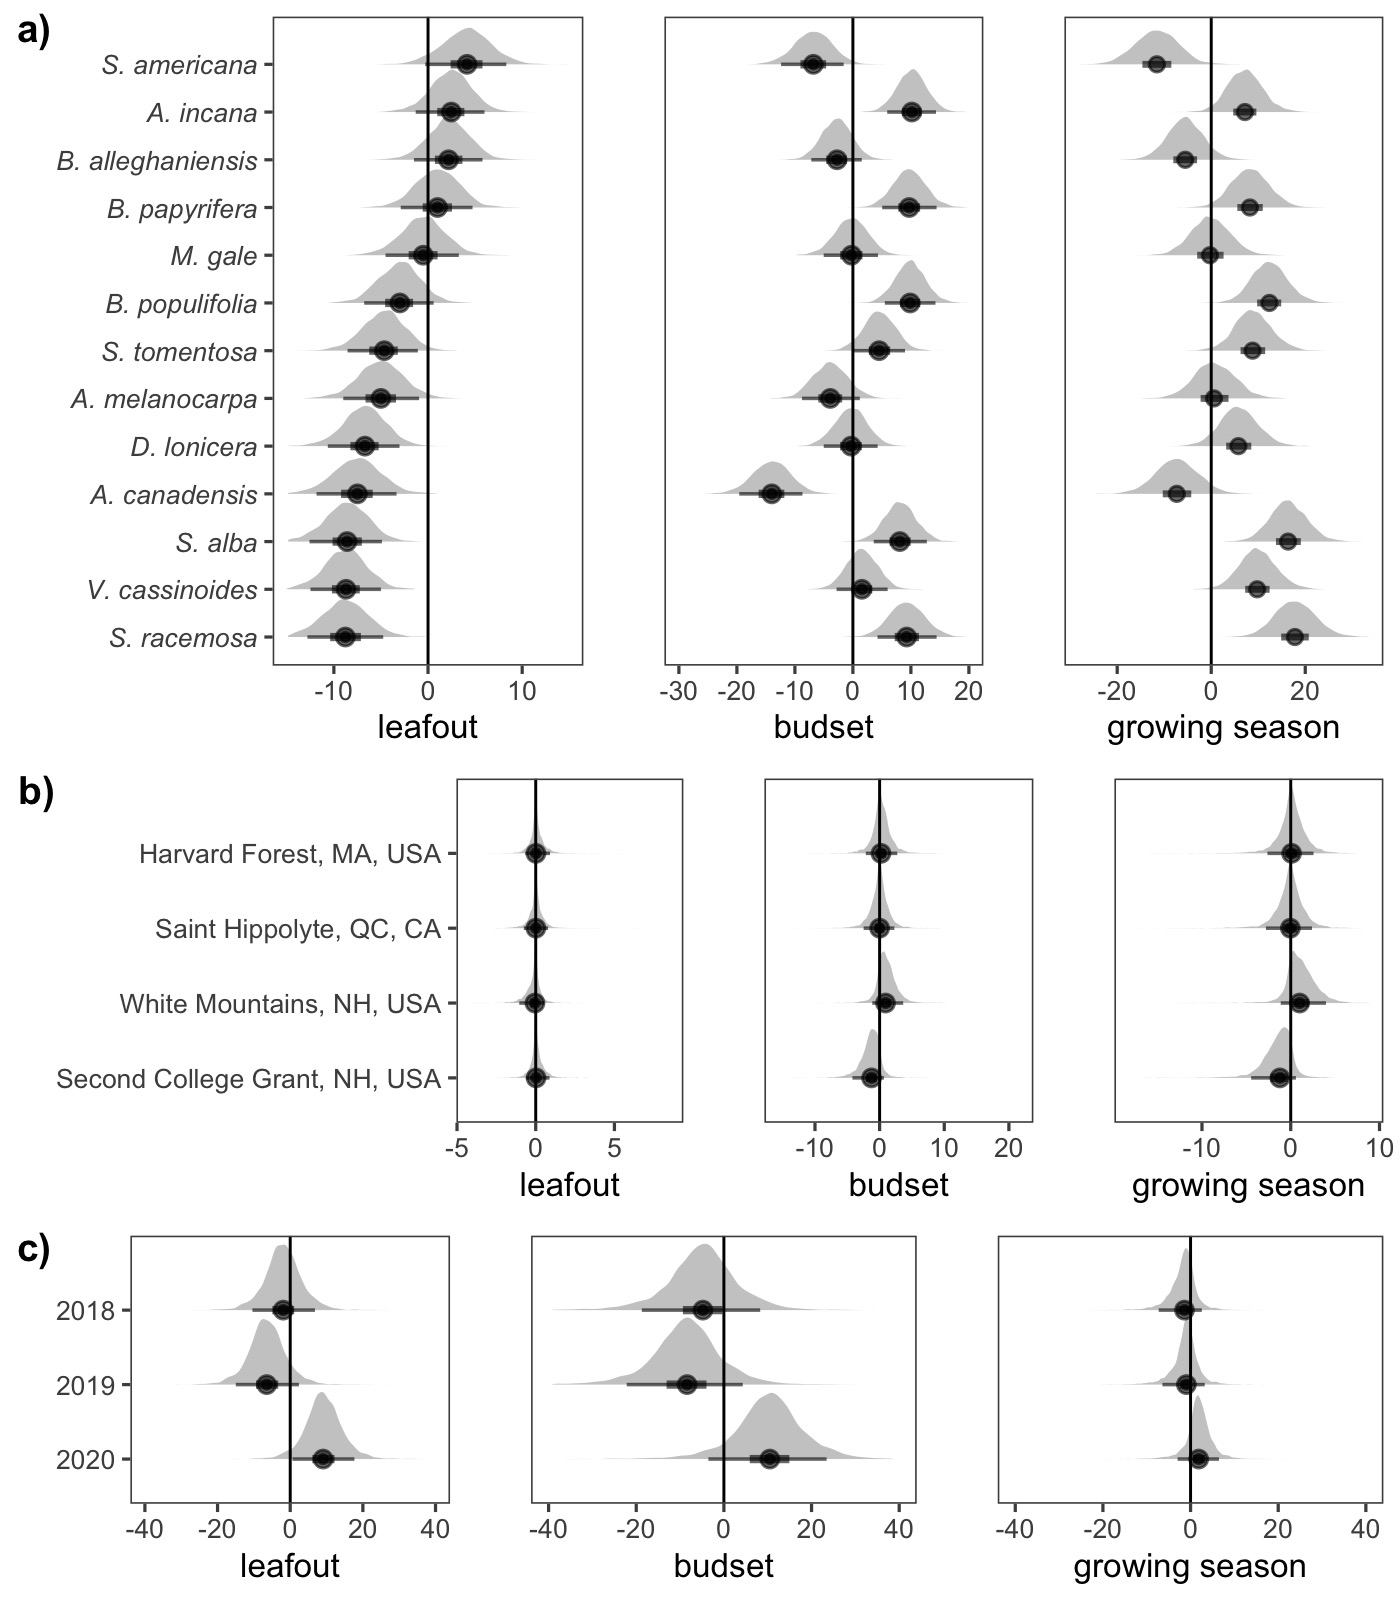
\includegraphics[width=.7\textwidth]{..//analyses/figures/var_parts.jpeg}
    \caption{Difference in leafout, budset and calendar growing season length partitioned between species (a) populations (b) and years (c). Point represent the median effect size estimate, and bars the 50\% uncertainty intervals. The grey distribution depict the full uncertainty estimate around the estimate.}
    \label{fig:vapar}
\end{figure}

%dl2024Sept20 such a cool result! 
%cjc2024Sept25 - agreed, this is awesome!
\begin{figure}[h!]
    \centering
 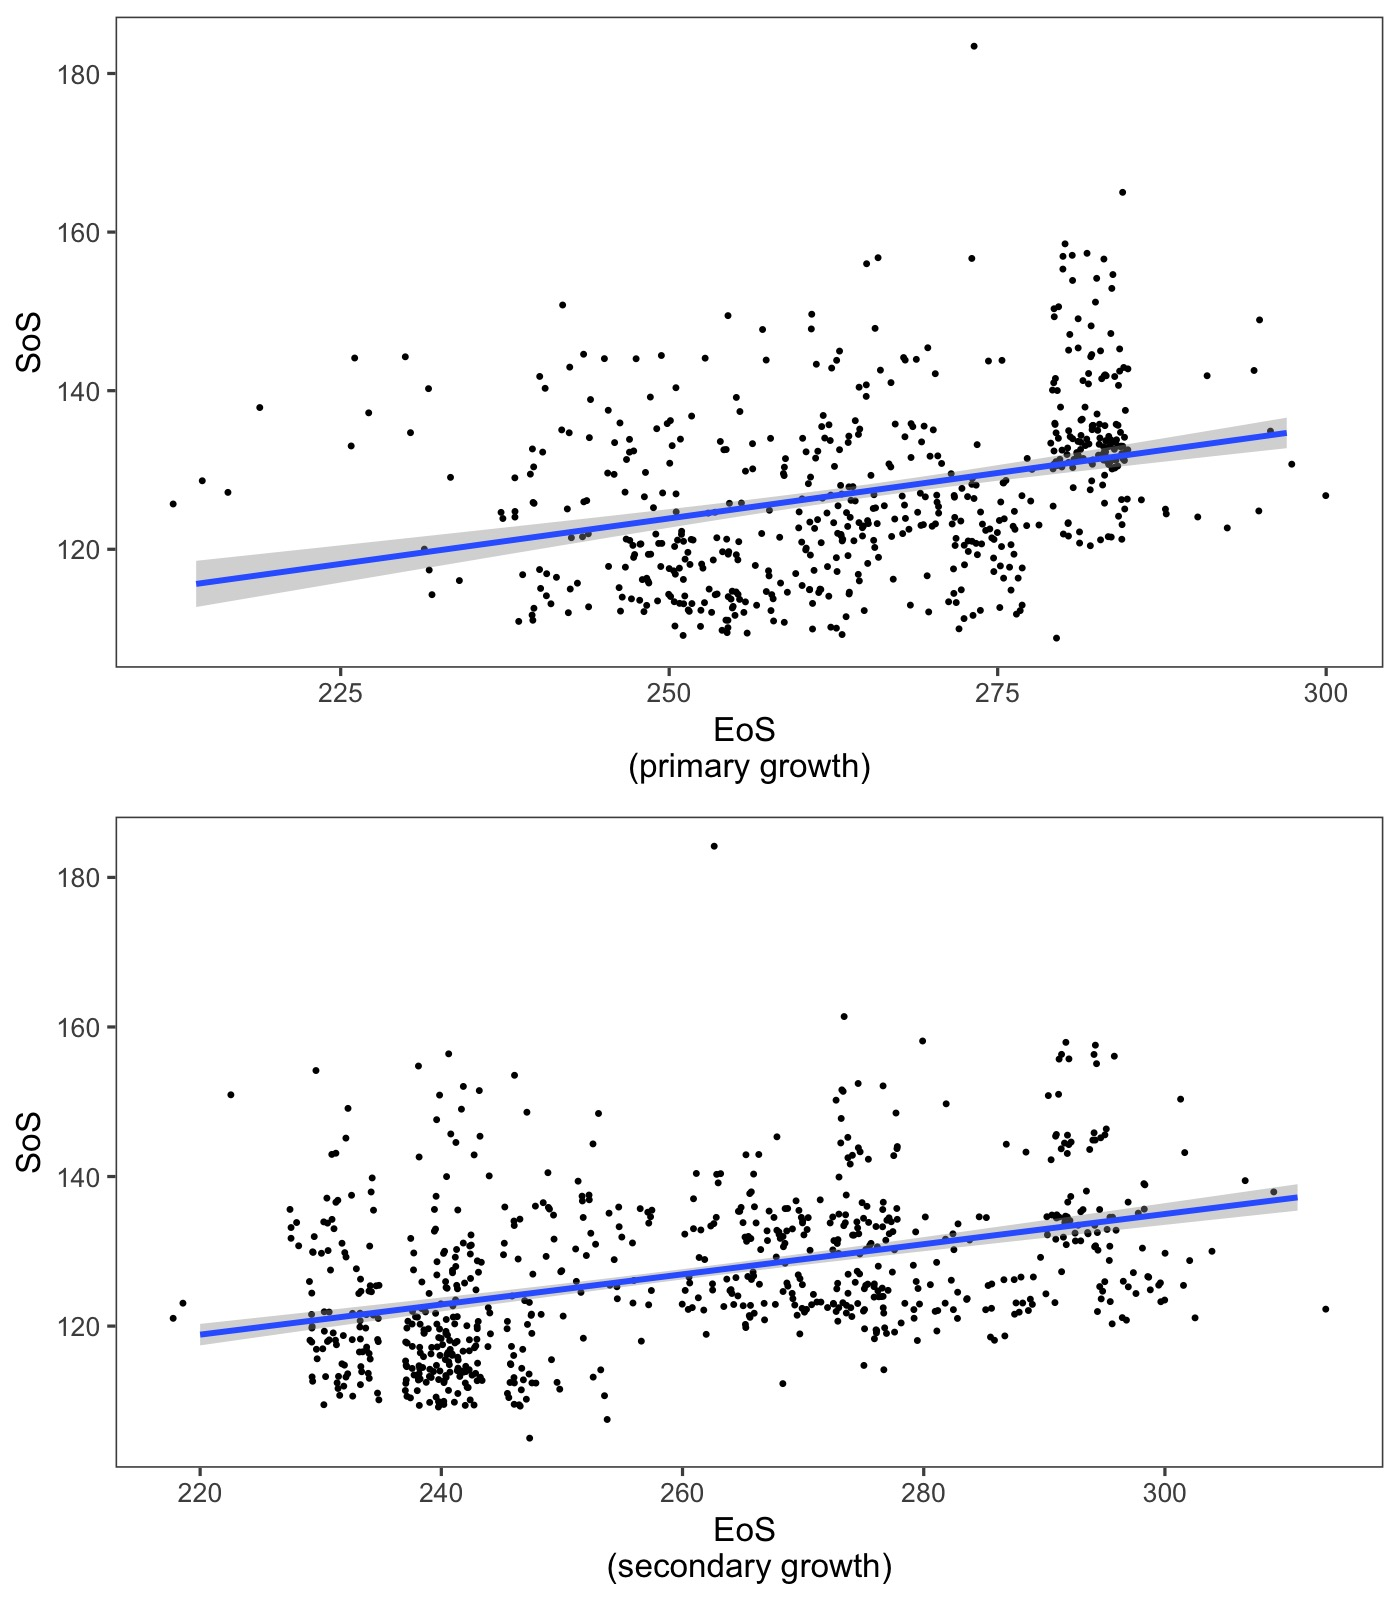
\includegraphics[width=.8\textwidth]{..//analyses/figures/primarygrowingseason_modplots.jpeg} % emwJuly22:  I love how few acronyms you use! Do you think we could delete them here and just mirror the language that main text? 
    \caption{The relationship between Start of Spring (SoS; calendar day of leafout) and growing season length differs between the calendar growing season and the thermal growing season. Later leafout resulted in a shorter calendar growing season (a) and this pattern was consistent across species in our study (b). In contrast, an increasing later SoS resulted in a longer thermal growing season (c) though this effect was stronger for species that typically leafout earlier in the season---panels in c) are display in the typical order of leafout among species. The blue trend lines represent the mean effect of SoS timing on growing season length and black lines represent 1000 draws from the posterior distribution as a measure of uncertainty. Points in a), and c) represent the raw data.}
    \label{fig:thermcal}
\end{figure}

%dl2024Sept20 can we add a legend defining the light and dark colors? I think the dark and light colors are switched in c.
%dl2024Sept20 I really like a, and what we are trying to show in b and c, but could see how the scale of the x-axis lessens the point we are trying to make.  Could we add some sort of transparent polygon in the background to show the thermal growing season and illustrate that the growth is outside of this window in b but not in c?
 \newpage
 \begin{figure}[h!]
    \centering
 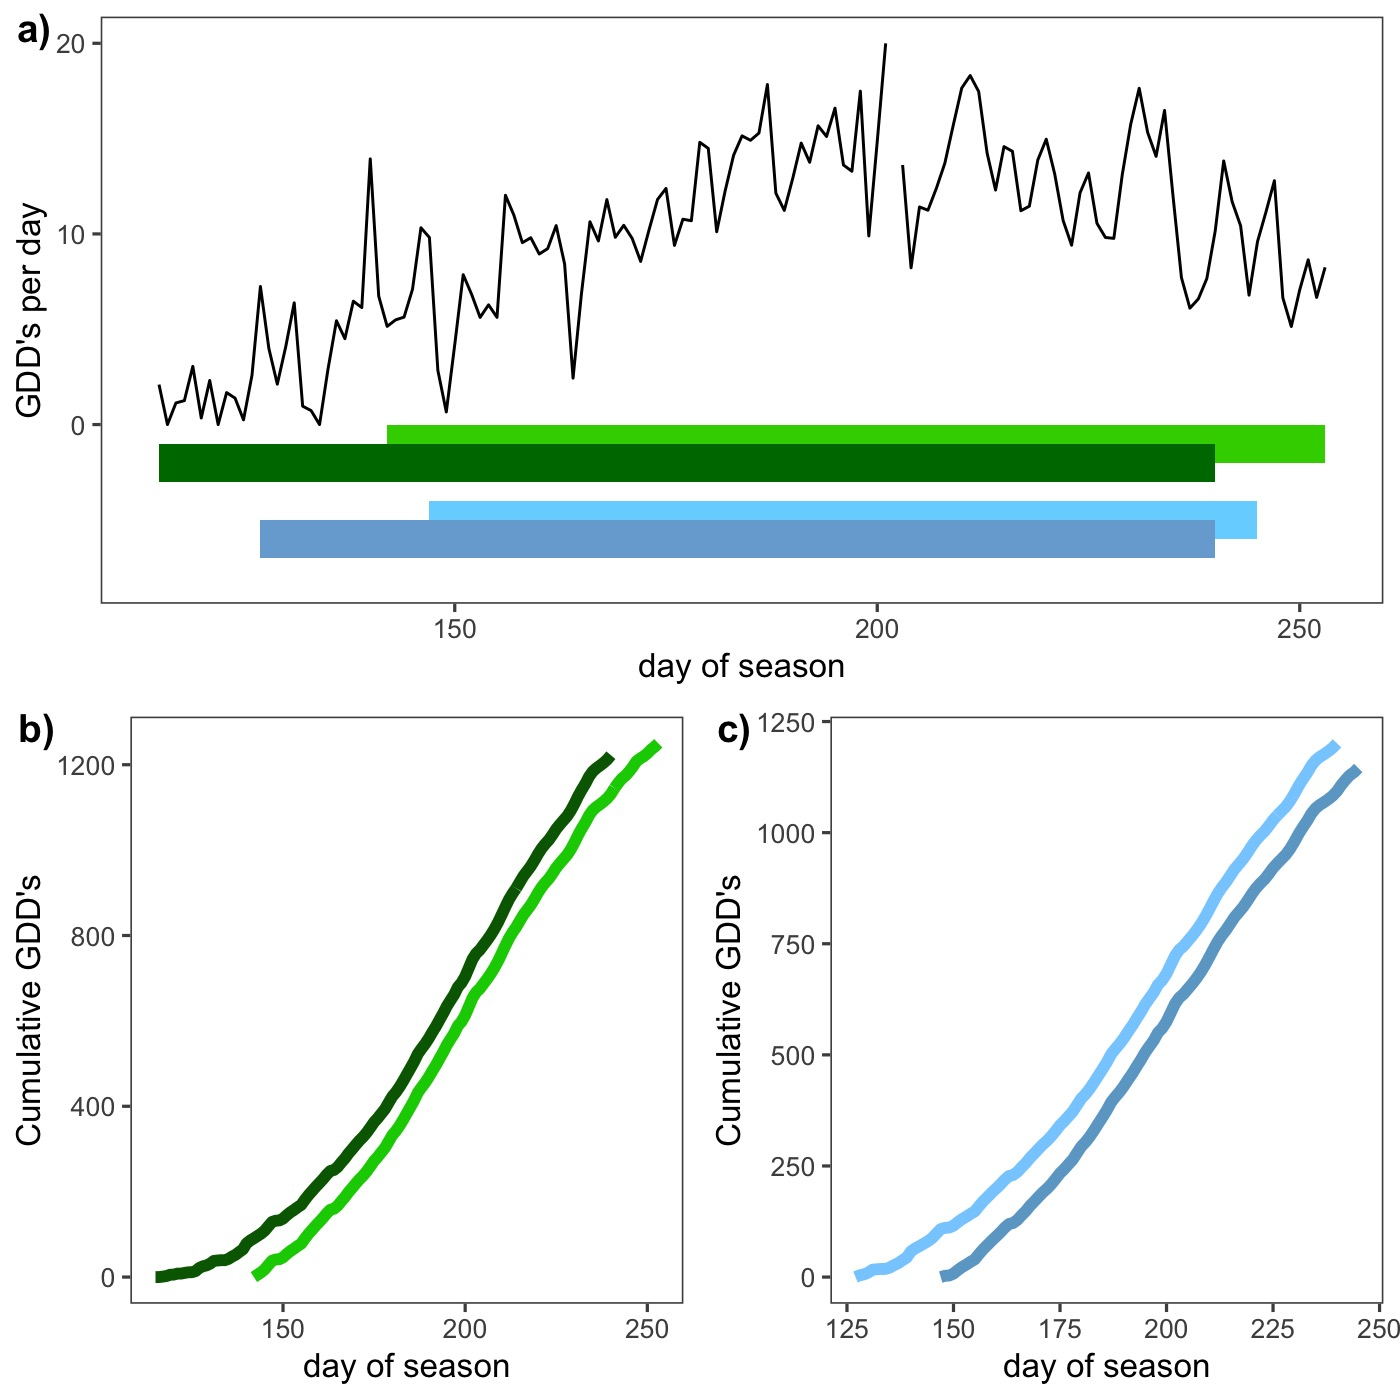
\includegraphics[width=.8\textwidth]{..//analyses/figures/aronia_examp.jpeg}
    \caption{Thermal conditions vary across the calendar growing season, which can generate a complex relationship between the calendar and thermal growing seasons. Panel a) depicts the daily heat sums at the Weld Hill Research Building in 2019 and the calendar growth season of early and late leafing individuals of \emph{Aronia melanocarpa} (green bars) and \emph{Myrica gale}(blue bars). Despite the fact the the early individual of \emph{A. melanocarpa} leafs out 24 days before it's later con-generic and only sets bud 13 days before it (i.e., it has a 14 day longer calendar growing season) it's thermal growing season is shorter (panel b) because most of its growth advantage (explain this better) takes place in the unfavorable early spring. In contrast for \emph{M. gale} where both the early and late individual leaf out later in the spring, the 20 day head start and 5 day earlier finish of the earlier individual (15 day longer calendar growing season) results in a longer thermal growing season for it as well (panel c)}.
    \label{fig:concept}
\end{figure}

\clearpage
% cjc2024Sept25: maybe we consider including sample sizes across the populations?
\begin{table}[ht] % emwJuly22: I second Cat's suggestion for the supp or such. I would also move this table to the supp and be sure you don't show species not in analysis or show clearly which are in or out (asterisk or something)? I would also add a little the caption that is in the methods about outplanting, which could save you a little methods text. 
\centering
\caption{Species list} 
\label{listSp}
\begin{tabular}{lrr}
  \hline
Species & functional group & n \\ 
  \hline
  \emph{Acer pensylvanicum} & tree  & 2 \\ 
  \emph{Acer spicatum} & tree & \emph{NA}  \\ 
   \emph{Alnus incana} & shrub & 31 \\ 
   \emph{Amelanchier canadensis} &  shrub & 6  \\ 
  \emph{Aronia melanocarpa} & shrub & 12 \\ 
  \emph{Betula alleghaniensis} &  tree & 24\\ 
  \emph{Betula papyrifera} &   tree & 13 \\ 
  \emph{Betula populifolia} &  tree & 24\\ 
  \emph{Diervilla lonicera} &  shrub  & 16 \\ 
  \emph{Myrica gale} &  shrub & 15\\ 
  \emph{Quercus alba} &  tree & \emph{NA}\\ 
  \emph{Quercus rubra} &  tree & \emph{NA}\\ 
  \emph{Sambucus racemosa} &  shrub & 11\\ 
  \emph{Sorbus americana} &  shrub & 5\\
  \emph{Spiraea alba} &  shrub & 19\\ 
  \emph{Spiraea tomentosa} &   shrub & 21 \\ 
  \emph{Vaccinium myrtilloides} &  shrub & \emph{NA}\\ 
  \emph{Viburnum cassinoides} &  shrub & 25 \\ 
  \end{tabular}
\end{table}


\newpage
\bibliography{..//refs/wildhell.bib}




\end{document}


